\documentclass[letterpaper, 12pt]{article}

%%%%%%%%%%%%%%%%%%%%%%%%%%%%%
% DEFINITIONS
% Change those informations
% If you need umlauts you have to escape them, e.g. for an ü you have to write \"u
\gdef\mytitle{Protokoll}
\gdef\mythema{DezSys08 - GPGPU}

\gdef\mysubject{Systemtechnik-DezSys}
\gdef\mycourse{5BHIT 2015/16}
\gdef\myauthor{Michael Weinberger}

\gdef\myversion{1.0}
\gdef\mybegin{15. Januar 2016}
\gdef\myfinish{23. Januar 2016}

\gdef\mygrade{Note:}
\gdef\myteacher{Betreuer: Borko/Micheler}
%
%%%%%%%%%%%%%%%%%%%%%%%%%%%%%

\input special/preamble.tex

\let\tempsection\section
\renewcommand\section[1]{\vspace{-0.3cm}\tempsection{#1}\vspace{-0.3cm}}
\WithSuffix\newcommand\section*[1]{\tempsection*{#1}}

\let\tempsubsection\subsection
\renewcommand\subsection[1]{\vspace{0cm}\tempsubsection{#1}\vspace{0cm}}

\let\tempsubsubsection\subsubsection
\renewcommand\subsubsection[1]{\vspace{0cm}\tempsubsubsection{#1}\vspace{0cm}}

\linespread{0.94}

\lhead{\mysubject}
\chead{}
\rhead{\bfseries\mythema}
\lfoot{\mycourse}
\cfoot{\thepage}
% Creative Commons license BY
% http://creativecommons.org/licenses/?lang=de
\rfoot{\ccby\hspace{2mm}\myauthor}
\renewcommand{\headrulewidth}{0.4pt}
\renewcommand{\footrulewidth}{0.4pt}

\begin{document}
\parindent 0pt
\parskip 6pt

\pagenumbering{Roman} 
%!TEX root=../laborprotokoll.tex

\begin{titlepage}

	\begin{figure}[!h]
		\begin{flushright}
			
\includegraphics[width=0.3\linewidth]{images/jdIT_tgm.png}
		\end{flushright}
	\end{figure}

	\vspace{2.5cm} 

	{\begin{center} \bfseries\huge
			\rule{17.5cm}{0.1mm}  
			\\[5mm]
			\mytitle\\[5mm]
			\mythema\\
			\rule{17.5cm}{0.1mm}  
	\end{center}}

	{\begin{flushright} \bfseries\Large
			\vspace{2cm}
			\mysubject\\
			\mycourse\\[10mm]
			\myauthor\\[10mm]
	\end{flushright}}

	{\begin{table}[!h] \bfseries\normalsize
		\begin{tabularx}{\textwidth}{lXr @{\hspace{0mm}}}
			&& Version \myversion\\
			\mygrade && Begonnen am \mybegin\\
			\myteacher && Beendet am \myfinish\\
		\end{tabularx}
	\end{table}}

\end{titlepage}


\clearpage
\thispagestyle{empty}
\tableofcontents

\newpage
\pagenumbering{arabic}
\pagestyle{fancy}

%\vspace{-0.5cm}
\section{Einführung}
\subsection{Ziele}
Die Aufgabe beinhaltet eine Recherche über grundsätzliche Einsatzmöglichkeiten für GPGPU. Dabei soll die Sinnhaftigkeit der Technologie unterstrichen werden. Die Fragestellungen sollen entsprechend mit Argumenten untermauert werden.
Im zweiten Teil der Arbeit soll der praktische Einsatz von OpenCL trainiert werden. Diese können anhand von bestehenden Codeexamples durchgeführt werden. Dabei wird auf eine sprechende Gegenüberstellung (Benchmark) Wert gelegt.
Die Aufgabenstellung soll in einer Zweiergruppe bearbeitet werden.

\subsection{Aufgabenstellung}
Informieren Sie sich über die Möglichkeiten der Nutzung von GPUs in normalen Desktop-Anwendungen. Zeigen Sie dazu im Gegensatz den Vorteil der GPUs in rechenintensiven Implementierungen auf [1Pkt]. \\
Gibt es Entwicklungsumgebungen und in welchen Programmiersprachen kann man diese nutzen [1Pkt]? \\
Können bestehende Programme (C/C++ und Java) auf GPUs genutzt werden und was sind dabei die Grundvoraussetzungen dafür [1Pkt]? \\ Gibt es transcompiler und wie kommen diese zum Einsatz [1Pkt]? \\

Präsentieren Sie an einem praktischen Beispiel den Nutzen dieser Technologie. Wählen Sie zwei rechenintensive Algorithmen (z.B. Faktorisierung) und zeigen Sie in einem aussagekräftigen Benchmark welche Vorteile der Einsatz der vorhandenen GPU Hardware gegenüber dem Ausführen auf einer CPU bringt (OpenCL). \\  \\ Punkteschlüssel: \\

Auswahl und Argumentation der zwei rechenintensiven Algorithmen (Speicher, Zugriff, Rechenoperationen) [0..4Pkt] \\
Sinnvolle Gegenüberstellung von CPU und GPU im Benchmark [0..2Pkt] \\
Anzahl der Durchläufe [0..2Pkt] \\
Informationen bei Benchmark [0..2Pkt] \\
Beschreibung und Bereitstellung des Beispiels (Ausführbarkeit) [0..2Pkt] \\

\subsection{Links}
OpenCL-Examples von René Hollander \& Paul Kalauner \cite{opencl_example}

\clearpage

\section{Möglichkeiten GPU Desktopanwendungen, Vorteil GPU bei rechenintensiven Implementierungen}
GPGPU (General Purpose Computation on Graphics Processing Unit) ist eine Programmier-Schnittstelle mit der Möglichkeit, allgemeine Berechnungen von der GPU ausführen zu lassen. Die ursprüngliche Aufgabe von Grafikchips ist, den Bildschirm mit Pixel zu füllen. Inzwischen eignen sich die umfangreichen Befehlssätze der GPUs auch für allgemeine Berechnungen, dies ist ein vergleichsweise neuer Trend in der Computertechnik, der darauf abzielt freie Rechenleistung konsequent auszunutzen. \\
Eine CPU besitzt wenige, im Serverbereich bis zu 16, Kerne die für jedmögliche Art von Berechnungen ausgelegt sind. Eine GPU besitzt mehrere Hundert, heute sogar schon bis zu über 1536 Kerne die parallel arbeiten. Ein Vorteil, bestimmte komplexe Berechnungen hierauf auszulagern erscheint klar sichtbar. 
\begin{figure}[!h]
	\begin{center}
		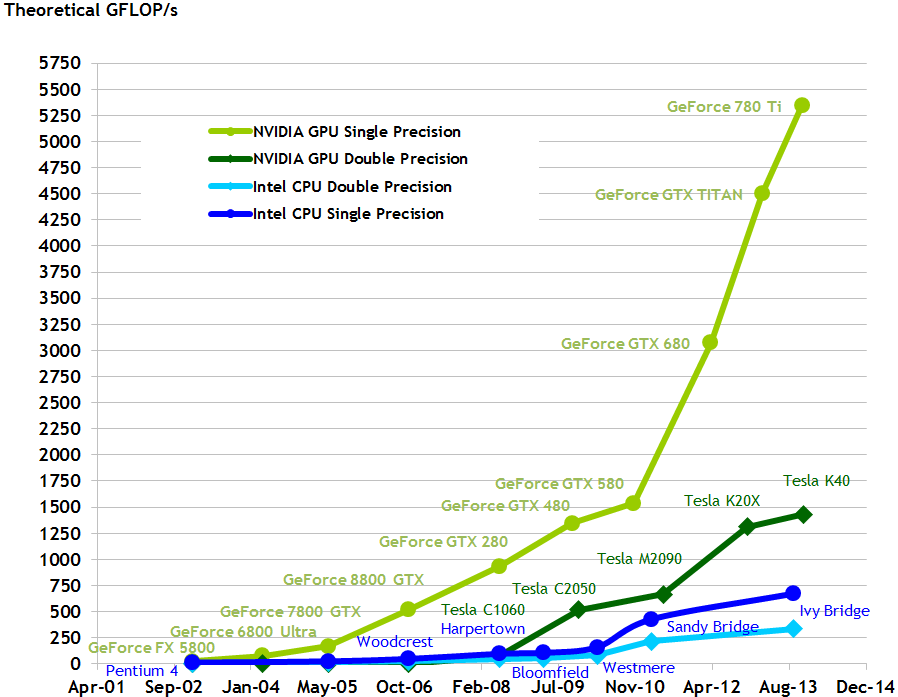
\includegraphics[width=1\linewidth]{images/floating-point-operations-per-second}
		\caption{GPU vs CPU, reine Rechenleistung \cite{comparison}}
		\label{Angabe}
	\end{center}
\end{figure}
Bei der reinen Rechenleistung ist wie auf dem Diagramm ersichtlich die GPU weit vorne. Die Rechenleistung ist in FLOPS (Floating Point Operations), die theoretisch mögliche Spitzenleistung, angegeben.

GPGPU wird verwendet um Rechenaufwendige Applikationen zu beschleunigen. Besonders aufwendig sind vor allem die folgenden Anwendungsbereiche Simulationswissenschaften, Medizin, Deep Learning. \\

Grafikkarten sind auf massive Parallelität ausgelegt, dies stellt aber auch Entwickler vor neue Herausforderungen. Es können je nach Anzahl an programmierbaren Shadereinheiten über 1000 Berechnungen zugleich in einem Takt ausgeführt werden. \cite{elko} \cite{Ausarbeitung}

\section{Entwicklungsumgebungen, Programmiersprachen}
\subsection{CUDA SDK}
Die CUDA Entwicklertools umfassen drei wichtige Komponenten: Den aktuellsten CUDA-Treiber, ein komplettes CUDA-Toolkit sowie CUDA SDK-Codebeispiele. In der Entwicklung bindet man ein Programm an den GPU-Hersteller Nvidia und somit an das Vorhandensein von Nvidia-Hardware. Es stellt eine umfassende Entwicklungsumgebung bereit, um hauptsächlich in C/C++ geschriebene Programme mithilfe der GPU zu beschleunigen. Es existieren aber auch Wrapper für die Sprachen Perl, Java, Python, Ruby, Fortran und .NET. \cite{cuda}

\subsection{OpenCL}
OpenCL (Open Computing Language) ist ein offenes, lizenzfreies und plattformübergreifendes Framework, um Systeme aus einer Kombination von CPUs, GPUs und anderen Prozessoren zu programmieren. OpenCL wurde ursprünglich von Apple entwickelt, und war der erste Standard, welcher nahezu perfekt für heterogene Systeme ausgelegt war. Eine namhafte Implementierung mithilfe von OpenCL ist etwa der APP SDK von AMD. Die Host-API ist in OpenCL C/C++ definiert, es gibt außerdem Third-Party-APIs für Python, Java und .NET. \cite{Ausarbeitung}

\section{Bestehende Programme (C/C++ und Java) auf GPUs nutzen und Grundvoraussetzungen}
Dies ist nur durch bestimmte Toolkits, wie etwa GPSME \cite{gpsme} möglich, das einem bestimmte Vorgänge abnimmt. Ansonsten ist dieser Schritt nicht ohne erheblichen Mehraufwand möglich, die Logik müsste bspw. in OpenCL C erneut geschrieben werden, was auch ein komplettes Redesign der Algorithmen zur parallelen Lauffähigkeit auf mehreren Kernen bzw. Threads mit sich zieht.

\newpage

\section{Transcompiler und deren Einsatz}
Nach einer Recherche ist mir kein solcher aufgefallen, der direkt source-to-source operiert. Wie im vorherigen Punkt beschrieben würde dies wahrscheinlich auch nur eingeschränkt Sinn machen, wenn z.B. Code in C ohne die benötigte Auslegung auf Parallelität zu OpenCL C-Code generiert wird. Außerdem sind in OpenCL C, welche im Grunde auf der Syntax von ISO C99 basiert, zusätzliche Datentypen und Funktionen enthalten zur parallelen Verarbeitung, die einem in C abgehen. Umso weiter entfernt scheint nun die Vorstellung eines Transcompilers, der hier alle Umstände berücksichtigt, und aus einer eingeschränkten Umgebung Code sinngemäß erweitern und verändern kann. \\
Zur generellen Erklärung: \\
Ein Transcompiler ist ein spezieller Compiler, der den Sourcecode eines Programmes in eine andere Programmiersprache überrträgt. \cite{transpiler}

\section{Praktisches Beispiel: Benchmark}
\subsection{Auswahl und Argumentation der Algorithmen}
\subsubsection{Pi berechnen auf beliebig viele Stellen mit GPUPI}
Die hier verwendete Bailey-Borwein-Plouffe-Formel ist eine Summenformel zur Berechnung der n-ten Nachkommazahl der Kreiszahl Pi. Der Gesamtaufwand beläuft sich auf die komplexe mathematische Berechnung.
\subsubsection{CompuBenchCL}
Die folgenden Tests werden im Benchmark berücksichtigt:
\begin{itemize}
	\item Gesichtserkennung \\
	Basiert auf dem Viola-Jones-Algorithmus, analysiert Bilder auf Gesichter, um biometrische Daten zu sammeln.
	\item  TV-L1 Optical Flow \\
	Dieses Berechnungsmodell wird etwa in der Vidokompression verwendet.
	\item Ocean Surface Simulation \\
	Testet den FFT-Algorithmus anhand von Meereswellen.
	\item Particle Simulation - 64k \\
	Simuliert viele einzelne Partikel in einem Würfel und deren Bewegungen.
	\item T-Rex \\
	Ein Kurzfilm als Echtzeitberechnung.
	\item Video Composition \\
	Stellt verschiedene Videofilter gleichzeitig dar.
	\item Bitcoin Mining \\
	Berechnen des Bitcoin-Algorithmus, die Hersteller werden sich freuen!
\end{itemize}

\newpage

\subsection{Gegenüberstellung CPU/GPU}
sadf
\subsection{Anzahl der Durchläufe}
sadf
\subsection{Informationen bei Benchmark}
Systemspezifikationen:
\begin{itemize}
	\item Acer Aspire V3-772
	\item Windows 8.1 64-bit
	\item Ausgabe 1920x1080p
	\item Intel Core i7-4702MQ @ 2.20Ghz, 4 Kerne, 8 logische Prozessoren
	\item NVIDIA GeForce GTX 760M \& Intel HD Graphics 4600 mit aktuellen Treibern (23.01.2016)
	\item CL API Intel OpenCL \& NVIDIA CUDA
	\item 16 GB RAM, 2 x 8 GB DDR3 1600 Mhz
	\item Toshiba-HDD, 1 TB
	\item Intel-SSD, 120 GB
	\item 100\%, Netzbetrieb
\end{itemize}
\subsection{Beschreibung, Bereitstellung des Beispiels}
sadf

\newpage

\bibliographystyle{unsrt}
\bibliography{DezSys08_Weinb_5BHIT}
\lstlistoflistings
\listoffigures

\end{document}
